\documentclass[a4paper,11pt]{article}
\usepackage{CLARIN2018}
% - - - - - - - IMPORTANT - - - - - - - -
% The next three lines allow XeLaTeX, graphics import and hyperlinks, set font and language
%\usepackage{xltxtra,polyglossia,graphicx,hyperref}
%\setmainfont[Mapping=tex-text]{Times}
%\setdefaultlanguage{english}
% If for some reason the above three lines are not compatible with your LaTeX installation,
% comment out the above three instructions and uncomment the following four instead:
\usepackage{times}
\usepackage{hyperref}
\usepackage{graphicx}
\usepackage{placeins}
\usepackage{enumitem}
%\usepackage{latexsym}
\usepackage[english]{babel}

%\setlength\titlebox{5cm}
\setlist{noitemsep}

% You can expand the titlebox if you need extra space
% to show all the authors. Please do not make the titlebox
% smaller than 5cm (the original size); we will check this
% in the camera-ready version and ask you to change it back.


\title{LaMachine: A meta-distribution for NLP software}

% - - - - - - - IMPORTANT - - - - - - -
% Leave the author information empty until your paper has been accepted

% Uncomment the following line ONLY if you need two author rows
%\setlength\titlebox{80mm}

\author{Maarten van Gompel  and Iris Hendrickx\\
  Centre for Language and Speech Technology (CLST) \\
  Radboud University, Nijmegen, the Netherlands \\
  {\tt proycon@anaproy.nl, i.hendrickx@let.ru.nl} \\ %\And % if needed: this makes a second column
  \url{https://proycon.github.io/LaMachine}
%  Second Author \\
%  Department (optional)\\
%  University Name without city \\
%  City, Country \\
% {\tt email@domain} \\
% \AND % if needed: this makes a second row
%  Third Author \\
%  Department (optional)\\
%  University of City, Country \\
%  {\tt email@domain} \\\And
%  Fourth Author \\
%  Department (optional)\\
%  University Name without city \\
%  City, Country \\
%  {\tt email@domain} \\
}

\date{}

\begin{document}
\maketitle

\begin{abstract}
We introduce LaMachine, a unified Natural Language Processing (NLP) open-source software distribution to facilitate the
installation and deployment of a large amount of software projects that have been developed in the scope of the
CLARIN-NL project and its current successor CLARIAH. Special attention is paid to encouragement of good software
development practices and reuse of established infrastructure in the scientific and open-source software development
community. We explain what Lamachine is, how it can be used and the technical details. We also compare Lamachine to alternative software distributions and discuss its advantages and limitations. We illustrate how LaMachine can be used in two case studies, one in an exploratory text mining project at the Dutch Health Inspectorate where LaMachine was applied to create a research environment for automatic text analysis for health care quality monitoring, and a second case where Lamachine was used to create a workspace for a one-week, intense collaboration by a diverse research team.
\end{abstract}

\section{Introduction}
\label{sec:intro}

Software is a key deliverable and a vital component for research in projects such as those under the CLARIN umbrella. Software provides researchers the instruments to yield for their research. It is CLARIN's core mission to make
digital language resources, including software, available to the wider research community.

We see that NLP software often takes on complex forms such as processing pipelines invoking various individual
components, which in turn rely on various dependencies. Add dedicated web-interfaces on top of that and you obtain a
suite of interconnected software that is often non-trivial to install, configure, and deploy. This is where LaMachine
comes in.

Software is a broad but well-ingrained notion in society nowadays, referring to any form of computer program. This can
manifest in various forms, whether it is an app on a phone, a graphical desktop application, a command line tool, or a
web-based application. These different \emph{interfaces} generally address different \emph{audiences}; the data
scientist will feel at home at the command line and in scripting environments and uses these fairly low-level
interfaces, whereas researchers in the humanities demand higher-level graphical interfaces. There is often a power trade-off
between lower and higher-level interfaces, with the former providing maximum flexibility at the cost of a steeper
learning curve, technical ability, and a do-it-yourself mentality. Higher level interfaces, on the other
hand, expose certain functionality of the software in an easy and accessible way, but in doing so often can not expose
the full power of the software. The cost trade-off is also apparant in the construction of the interfaces, where
high-level interfaces are typically far more costly to build.

LaMachine incorporates software providing different types of interfaces which, as seen above, typically address different audiences. Whilst we
attempt to accommodate both technical\footnote{Data scientists, DevOps, system administrators, developers.} and
less-technical audiences\footnote{The wider researcher community, particularly the Humanities; also educational
settings.}, there is a natural bias towards the former as lower-level interfaces are often a prerequisite to build
higher-level interfaces on. Depending on the \emph{flavour} (more on this later) of LaMachine chosen, it makes a good virtual research
environment for a data scientist, whether on a personal computer or on a computing cluster, a good development
environment for a developer or a good deployment method for production servers in for example CLARIN centres.

 This paper provides a detailed description of Lamachine, its purpose and functionality and the technical details. We
 discuss the advantages and limitations of LaMachine compared to alternative software distributions in Section \ref{sec:comparison}. We demonstrate how LaMachine can create a fully functioning and standalone research environment for text mining  and NLP for Dutch texts in two use cases in Section \ref{sec:case}.

 \section{What is Lamachine?}

LaMachine is an open-source NLP software distribution.  LaMachine facilitates the installation, distribution and configuration of software. It does not fork, modify or appropriate the participating software in any way, nor does it provide a hosting place or repository for software.
We classify LaMachine as a \emph{meta distribution} as it can be installed in various contexts. The heart of LaMachine consists of a
set of machine-parsable instructions on how to obtain, build (e.g. compile from source), install and configure software.
%iris:  eerst algemene uitleg over lamachine- dit is veel te gedetaileerd op dit punt-
%These are implemented using Ansible\footnote{\url{https://www.ansible.com}; a popular open-source software provisioning,
%configuration and deployment tool by Red Hat}.
This is notably different from the more
classical notion of Linux distributions, which generally provide their own repositories with (often binary) software
packages. LaMachine builds on this already established infrastructure by taking these repositories as a foundation where
possible. Similarly, as implied in point five above, there are different programming-language-specific ecosystems
providing their own repositories, such as the Python Package Index\footnote{\url{https://pypi.org}} for Python,
CRAN\footnote{\url{https://cran.r-project.org/}} for R, CPAN\footnote{\url{https://www.cpan.org}} for Perl, Maven
Central\footnote{\url{https://search.maven.org}} for Java.  LaMachine relies on those to obtain and install software. In doing so, we compel participating software projects
to adhere to well-established distribution standards and ensure the software is more sustainable towards the future
\cite{softwarequality}. Moreover, we ensure that LaMachine never becomes a prerequisite for the software but merely a
courtesy or convenience, and attempt to limit any amount of duplication in packaging and distribution efforts.

LaMachine lives in an open-source ecosystem and therefore builds on Unix-like platforms; this primarily means Linux, as well as BSD and, with some restrictions, macOS. This by definition excludes certain software for different platforms, such as mobile platforms (Android/iOS/etc), native Windows/mac desktop applications, or certain interface types in general such as classical desktop GUI applications or mobile `apps', all of which fall beyond our scope. Cygwin\footnote{A unix environment on Windows} is not tested or
 supported either. However, virtualisation technology enables deployment on a wider range of platforms, including Windows.


The software included in LaMachine has to adhere to the following prerequisites:

\begin{enumerate}

    \item The software must have a recognised (i.e. OSI-approved) open-source license.
        Proprietary (closed-source) software is explicitly excluded.
    \item The source
        code must be hosted in a public version controlled repository.\footnote{e.g. Github, Gitlab, Bitbucket, provided
        the respository is public}
    \item There must be a build process to compile the source, if applicable, and install the program or library.
    \item There must be some kind of release protocol (adhering to semantic versioning) that publishes software using the proper
technology-specific channels. We will elaborate on this later.
    \item All software that is incorporated in LaMachine must bear at least some relevance to the field of Natural Language Processing.
    \item Participating software must be actively maintained (i.e. not outdated or abandoned) and not place any demands on outdated
        dependencies. %verwerkt <-- maarten help even met formuleren hier, ik bedoel dat zoiets als Pattern dus helaas niet mee kan doen omdat het niet meer onderhouden wordt }only maintained/uptodate date software that can compile using the current version of compilers and dependencies/libraries
\end{enumerate}


\section{ Included Software}

LaMachine exists since May 2015 and has been used extensively ever since by numerous users. In early 2018 version 2 was
released which was a significant redesign, powered by Ansible\footnote{\url{https://www.ansible.com}}.

In LaMachine, software is grouped into various ``packages'', each package\footnote{For those familiar with
Ansible, a package in LaMachine is an Ansible role} groups one or multiple programs that have some kind of relation. The
installation manifest lists all packages that will be installed, at the user's discretion. After the initial
installation, the user can always add more packages using \texttt{lamachine-add} or editing the installation manifest directly.

LaMachine was initially conceived as the primary means of distribution of the software stack developed at the Language
Machines Research Group and the Centre of
Language and Speech Technology, Radboud University Nijmegen. The majority of this sofware was either fully or partially developed under the auspices of CLARIN-NL or successor
CLARIAH. Some software by other CLARIN-NL/CLARIAH partners is also included. LaMachine is not limited to one research
group and is explicitly open to participation by other software providers, especially those
also in CLARIAH.

We list a selection of the most important software included in LaMachine, grouped by research institute:

\begin{itemize}
 \item by the Language Machines Research Group and the Centre of Language and Speech Technology, Radboud University,
     Nijmegen\footnote{Links: \url{https://languagemachines.github.io/timbl}, \url{https://languagemachines.github.io/mbt},
    \url{https://languagemachines.github.io/ucto}, \url{https://languagemachines.github.io/frog},
    \url{http://ilk.uvt.nl/wopr}, \url{https://proycon.github.io/folia}, \url{https://proycon.github.io/clam},
\url{https://github.com/proycon/flat}, \url{https://proycon.anaproy.nl/pynlpl},
\url{https://proycon.github.io/colibri-core/},
\url{https://github.com/proycon/gecco},
\url{https://github.com/proycon/valkuil-gecco},
\url{https://github.com/LanguageMachines/PICCL}, \url{https://github.com/LanguageMachines/ticcltools},
\url{https://github.com/proycon/labirinto},
\url{https://github.com/proycon/oersetter-webservice}
}
 \begin{itemize}
     \item \textbf{Timbl} -- A memory-based machine learning
         toolkit, and \textbf{Mbt}, a memory-based tagger based on timbl. Python bindings included as well.
     \item \textbf{Ucto} -- A multilingual rule-based tokeniser. Python binding included as well.
     \item \textbf{Frog} -- An integration of various memory-based natural language processing (NLP) modules
         developed for Dutch. It can do Part-of-Speech tagging, lemmatisation, named entity recogniton, shallow parsing,
         dependency parsing and morphological analysis. Also included in LaMachine;
         Python bindings for Frog and \textbf{Toad}, Trainer Of All Data, training tools for Frog.
     \item \textbf{Wopr} -- Memory-based Word Predictor.
     \item \textbf{CLAM} -- Quickly build RESTful webservices, powers many webservices offered by LaMachine.
     \item \textbf{FoLiA} -- Format for Linguistic Annotation \cite{FOLIAPAPER}, with tools and libraries in/for Python and $C++$.
     \item \textbf{FLAT} -- FoLiA Linguistic Annotation Tool: a web-based linguistic annotation tool.
     \item \textbf{PyNLPl} -- Python Natural Language Processing Library.
     \item \textbf{Colibri Core} -- Colibri core is an NLP tool as well as a C++ and Python library for working with
         basic linguistic constructions such as n-grams and skipgrams (i.e patterns with one or more gaps, either of
         fixed or dynamic size) in a quick and memory-efficient way.
     \item \textbf{Gecco} -- Generic Environment for Context-Aware Correction of Orthography, an NLP pipeline for
         spelling correction,  and \textbf{Valkuil.net}, an instantiation thereof for Dutch.
     \item \textbf{PICCL} -- A set of workflows (NLP pipeline) for corpus building through OCR, post-correction (through \textbf{TICCL}) and Natural Language Processing.
     \item \textbf{Labirinto} -- A web-based portal listing all
         available tools in LaMachine, an ideal starting point for LaMachine.
     \item \textbf{Oersetter} -- A Frisian-Dutch Machine Translation system in collaboration with the Fryske Akademy.
 \end{itemize}
 \item by the University of Groningen
 \begin{itemize}
     \item \textbf{Alpino}\footnote{\url{http://www.let.rug.nl/vannoord/alp/Alpino/}} - A dependency parser and tagger for Dutch.
 \end{itemize}
 \item by the Vrije Universiteit Amsterdam
 \begin{itemize}
     \item \textbf{KafNafParserPy}\footnote{\url{https://github.com/cltl/KafNafParserPy}} - A python module to parse NAF files.
 \end{itemize}
 \item by Utrecht University
 \begin{itemize}
     \item  \textbf{T-scan}\footnote{\url{https://github.com/proycon/tscan}} - T-scan is a Dutch text analytics tool for readability prediction (initially developed at TiCC, Tilburg University, and in collaboration with Radboud University, Nijmegen)
 \end{itemize}
 \item by the Meertens Instituut
 \begin{itemize}
     \item \textbf{Python Course for the Humanities}\footnote{\url{http://www.karsdorp.io/python-course/}} - Interactive
         tutorial and introduction into programming with Python for the humanities.
 \end{itemize}
\end{itemize}

In addition to the above listed specific software, LaMachine also incorporates a large number of renowned tools by external international parties, offering
most notably a mature Python environment with scientific modules. The following list gives an impression and is not
exhaustive: \footnote{Links: \url{https://jupyterlab.readthedocs.io/en/stable/}, \url{https://pytorch.org}, \url{http://www.nltk.org},
    \url{https://spacy.io},  \url{http://www.nextflow.io}, \url{https://stanfordnlp.github.io/CoreNLP/},  \url{https://github.com/tesseract-ocr/tesseract}, \url{https://tensorflow.org},
\url{http://kaldi-asr.org}, \url{http://www.statmt.org/moses}}

\begin{itemize}
    \item \textbf{Python}: Numpy, Scipy, Matplotlib, Scikit-Learn, IPython, Jupyter, ...
    \begin{itemize}
        \item \textbf{Jupyter Lab} The successor of the popular Jupyter Notebooks, offers notebooks, a web-based IDE, terminals. An ideal entry point to get started with LaMachine and all it contains!
        \item \textbf{PyTorch} - Deep-learning library for Python
        \item \textbf{NLTK} - Natural Language Toolkit for Python
        \item \textbf{Spacy} - Industrial-Strength NLP in Python
    \end{itemize}
    \item \textbf{R}
    \item \textbf{Java}
    \begin{itemize}
        \item \textbf{NextFlow} - A system and language for writing parallel and scalable pipelines in a portable manner.
        \item \textbf{Stanford CoreNLP} - Various types of linguistic enrichment
    \end{itemize}
    \item \textbf{Tesseract} - Open Source Optical Character Recognition (OCR)
    \item \textbf{Tensorflow} - Open-source machine learning framework
    \item \textbf{Kaldi} - Speech Recognition Framework (ASR)
    \item \textbf{Moses} - Statistical Machine Translation system
\end{itemize}



\section{Architecture}

In this section we present the technical design choices that were made and lay out the architecture of LaMachine.
%iris: Maarten je zou hier ook expliciet de motivatie voor de keuzen kunnen toevoegen

\subsection{Flavours}

LaMachine provides ample flexibility that allows it to be deployable in different contexts. First of all there is
flexibility regarding the installation form, which we call \emph{flavours}:

\begin{enumerate}
    \item \textbf{Local installation} -- This installs the bulk of LaMachine in a separate local virtual environment (a seperate
        directory\footnote{Python users should know we just use \texttt{virtualenv} for this, with some
        additions of our own}) that has to be explicitly activated to be used. This also allows for multiple different installations
        of LaMachine on the same host system (e.g. for different users or with different software configurations).
        This local installation still actively relies on various global dependencies that are available through the
        package manager of your distribution.
    \item \textbf{Global installation} -- This flavour is used for a host that is fully dedicated to LaMachine. Everything will be
        installed globally so there is only one installation possible, multiple users will all make use of the same
        installation. Unlike the local installation, we do not make use of a Python Virtual Environment in this flavour.
    \item \textbf{Docker container} -- Installs LaMachine in a container. Containerisation separates the entire run-time
        environment from the host system, only the Linux kernel is shared. It is a lighter option than full
        virtualisation. \footnote{Note that Docker on other platforms such as Windows and macOS does do use full
        virtualisation.}
    \item \textbf{Singularity container} -- Another form of containerisation with more focus on security\footnote{reduced
        privilege escalation}, making it more suitable than Docker for deployment on computing clusters. This flavour is still under development.
    \item \textbf{Virtual Machine} --- Installs LaMachine as a virtual machine, i.e. through full virtualisation. This allows
        deployment of LaMachine on hosts which would otherwise not support it, such as Windows. Virtualisation for
        LaMachine is achieved through Vagrant and VirtualBox\footnote{\url{https://vagrant.org}, \url{https://www.virtualbox.org}}.
    \item \textbf{Remote provisioning} -- Installs LaMachine on a remote dedicated server. This option is most suited for
        hosting centres and directly uses Ansible's remote provisioning abilities.
\end{enumerate}

The different flavours all offer a different degree of separation from the host OS, where Virtual Machines are
completely virtualised, containers still share the kernel with the host OS, and the two native installation flavours,
local and global, actually compile against the machine's distribution itself and thus offer the least amount of
overhead.

The two native options support a variety of major GNU/Linux distributions: Debian, Ubuntu, Arch Linux, CentOS, Fedora
and, to a more limited degree, we also support macOS, powered in part by the homebrew package
manager\footnote{\url{https://brew.sh}; alternatives such as macports are not supported}. Support for macOS is limited because not all participating
software supports it. Certain Linux Distributions that are derivatives of the aforementioned distributions \emph{may} also work, such as RedHat
Enterprise Linux (CentOS) and Linux Mint (Ubuntu).

For the containerisation and virtualisation solutions, the default distribution we supply is Debian\footnote{The latest
stable release}. It is, however, still possible to build your own container or virtual machine based on any of the other supported
distributions. In fact, containers, virtual machines and remote provisioning can all be considered special wrapped forms of
the global installation flavour.

Pre-built docker containers and virtual machine images with a limited selection of participating software are uploaded
to the Docker Hub\footnote{\url{https://hub.docker.com/r/proycon/lamachine/}} and Vagrant
Cloud\footnote{\url{https://app.vagrantup.com/proycon/boxes/lamachine}}, respectively, for each LaMachine release.

\subsection{Versions}

LaMachine offers three distinct \emph{versions}, regardless of the flavour:

\begin{enumerate}
    \item \textbf{stable} - This is the default and recommended for most situations. It installs the latest stable
        versions of all included software.
    \item \textbf{development} - This installs the latest development versions of the included software. In practise,
        this usually means that software is pulled directly from the version-controlled repository is and compiled and installed from source. Due to the experimental nature, the development version of
        LaMachine may at times break and not install successfully.
    \item \textbf{custom} - This installs custom versions of all included software, i.e. the user explicitly
        specifies which versions to install for each software package.  Such a version list can for instance be exported
        from another LaMachine installation, and then allows to rebuild a similar environment from scratch, providing a
        limited level of reproducibility. We say limited, because packages
        provided by the underlying distribution are not a part of this scheme.
\end{enumerate}

The nomenclature is admittedly a bit confusing, but the notion of version discussed in this section refers to the
versions of the various software packages inside LaMachine. It should not be
confused with the actual \emph{version release number} of Lamachine as a whole, which is the version number assigned to
the collective of installation scripts LaMachine provides, and which marks LaMachine releases.

\subsection{Bootstrapping}

Installation of LaMachine begins with a single \emph{bootstrap} command\footnote{See \url{https://proycon.github.io/LaMachine}}
executed on the command line.  It can interactively query the user for her software preferences \emph{(stored as the
host configuration)}, e.g. the flavour of LaMachine, as well as the set of software to install, \emph{the installation
manifest}. This set is never static but can be customised by the user. The bootstrap procedure, a screenshot of which is shown in
Figure~\ref{fig:bootstrap}, detects and installs the
necessary prerequisites automatically and eventually invokes Ansible to perform the bulk of the work, unless a
pre-published container or VM is selected.  Figure~\ref{fig:arch} provides a schematic view of the LaMachine
architecture.

\begin{figure}[htb] \begin{center}
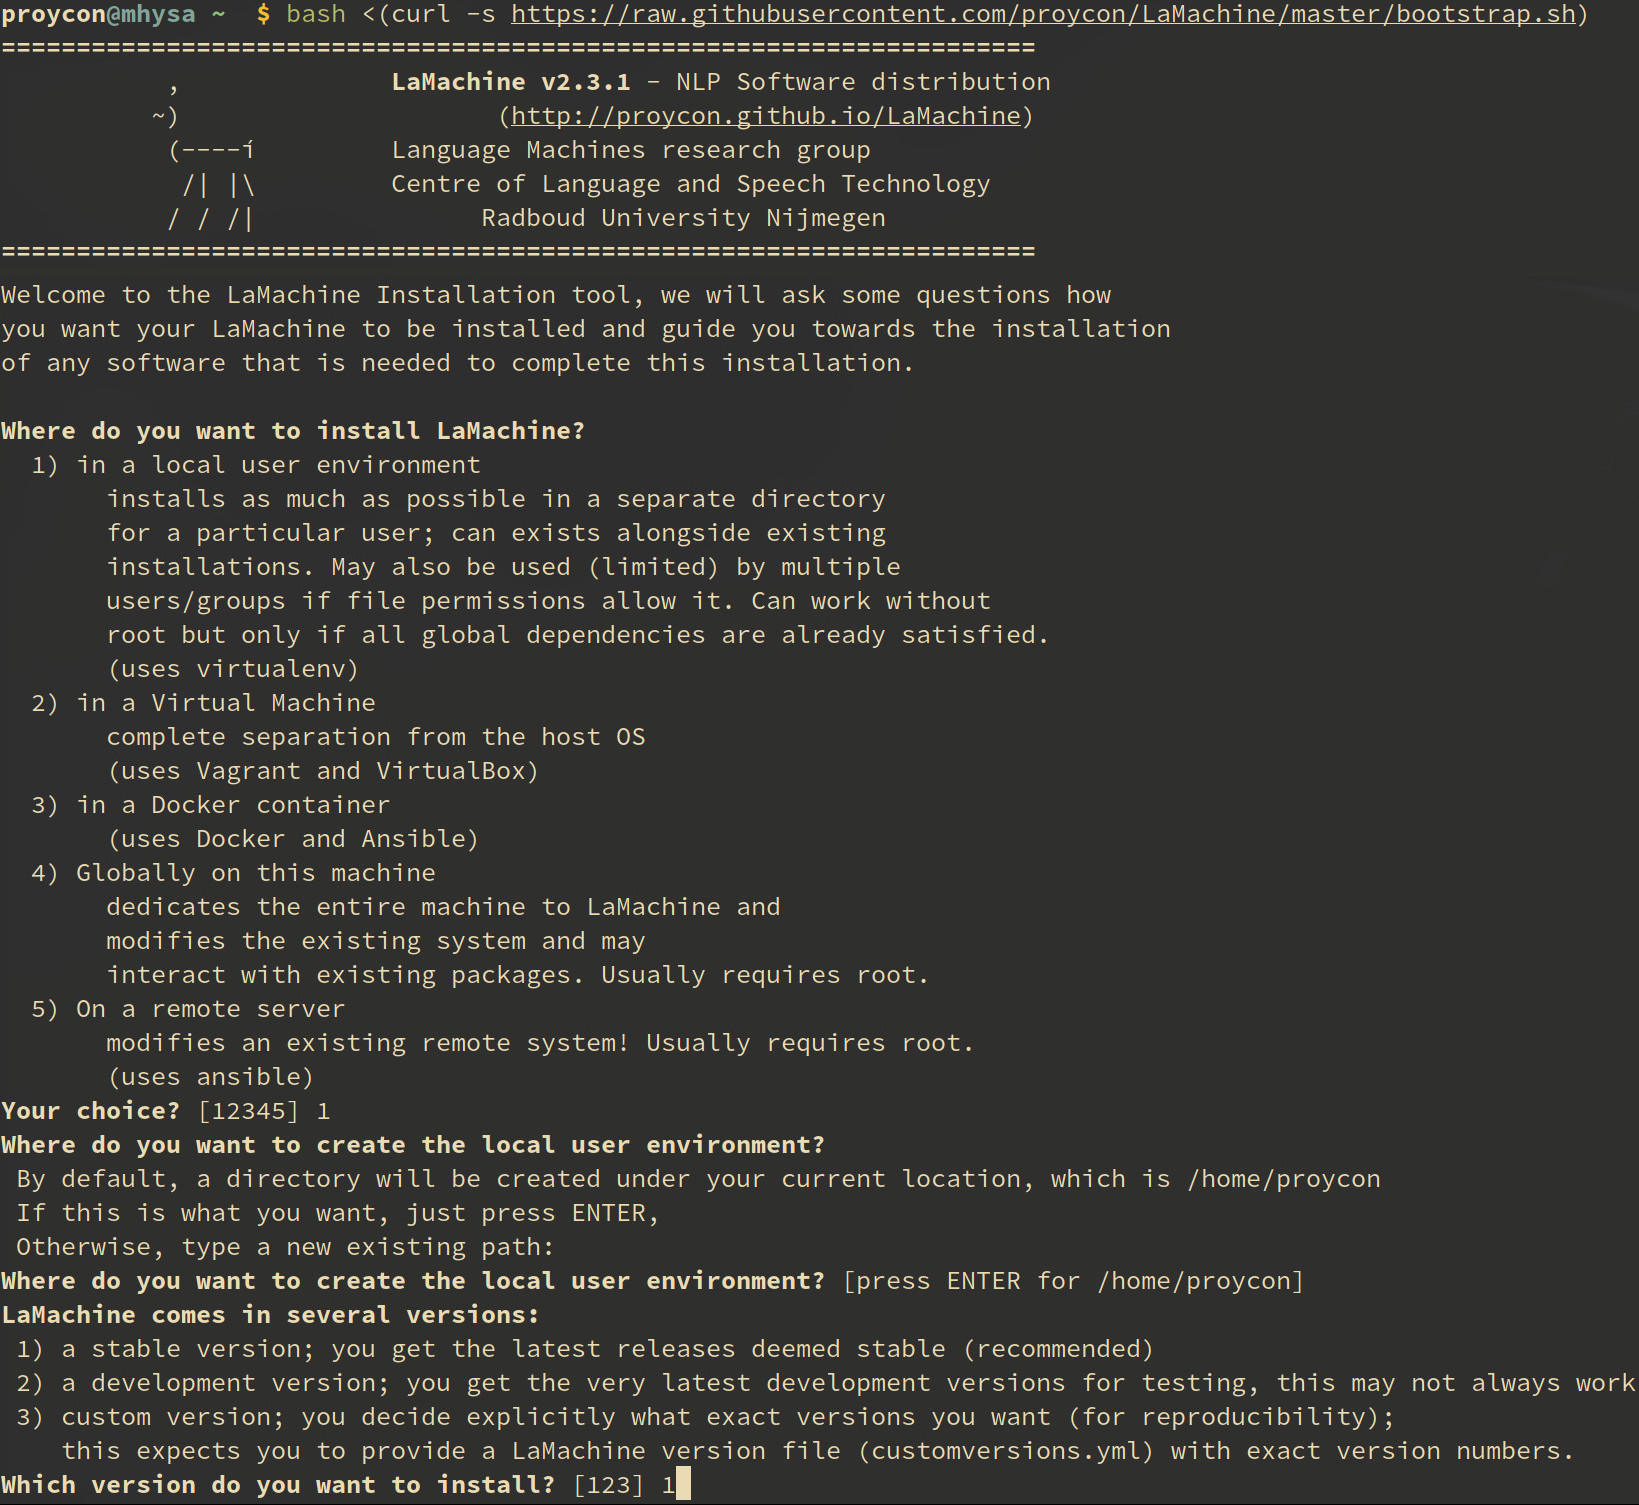
\includegraphics[width=110.0mm]{screenshot_bootstrap.jpg}
\end{center}
\caption{\footnotesize{A screenshot of the bootstrap procedure}}
\label{fig:bootstrap}
\end{figure}

\begin{figure}[htb] \begin{center}
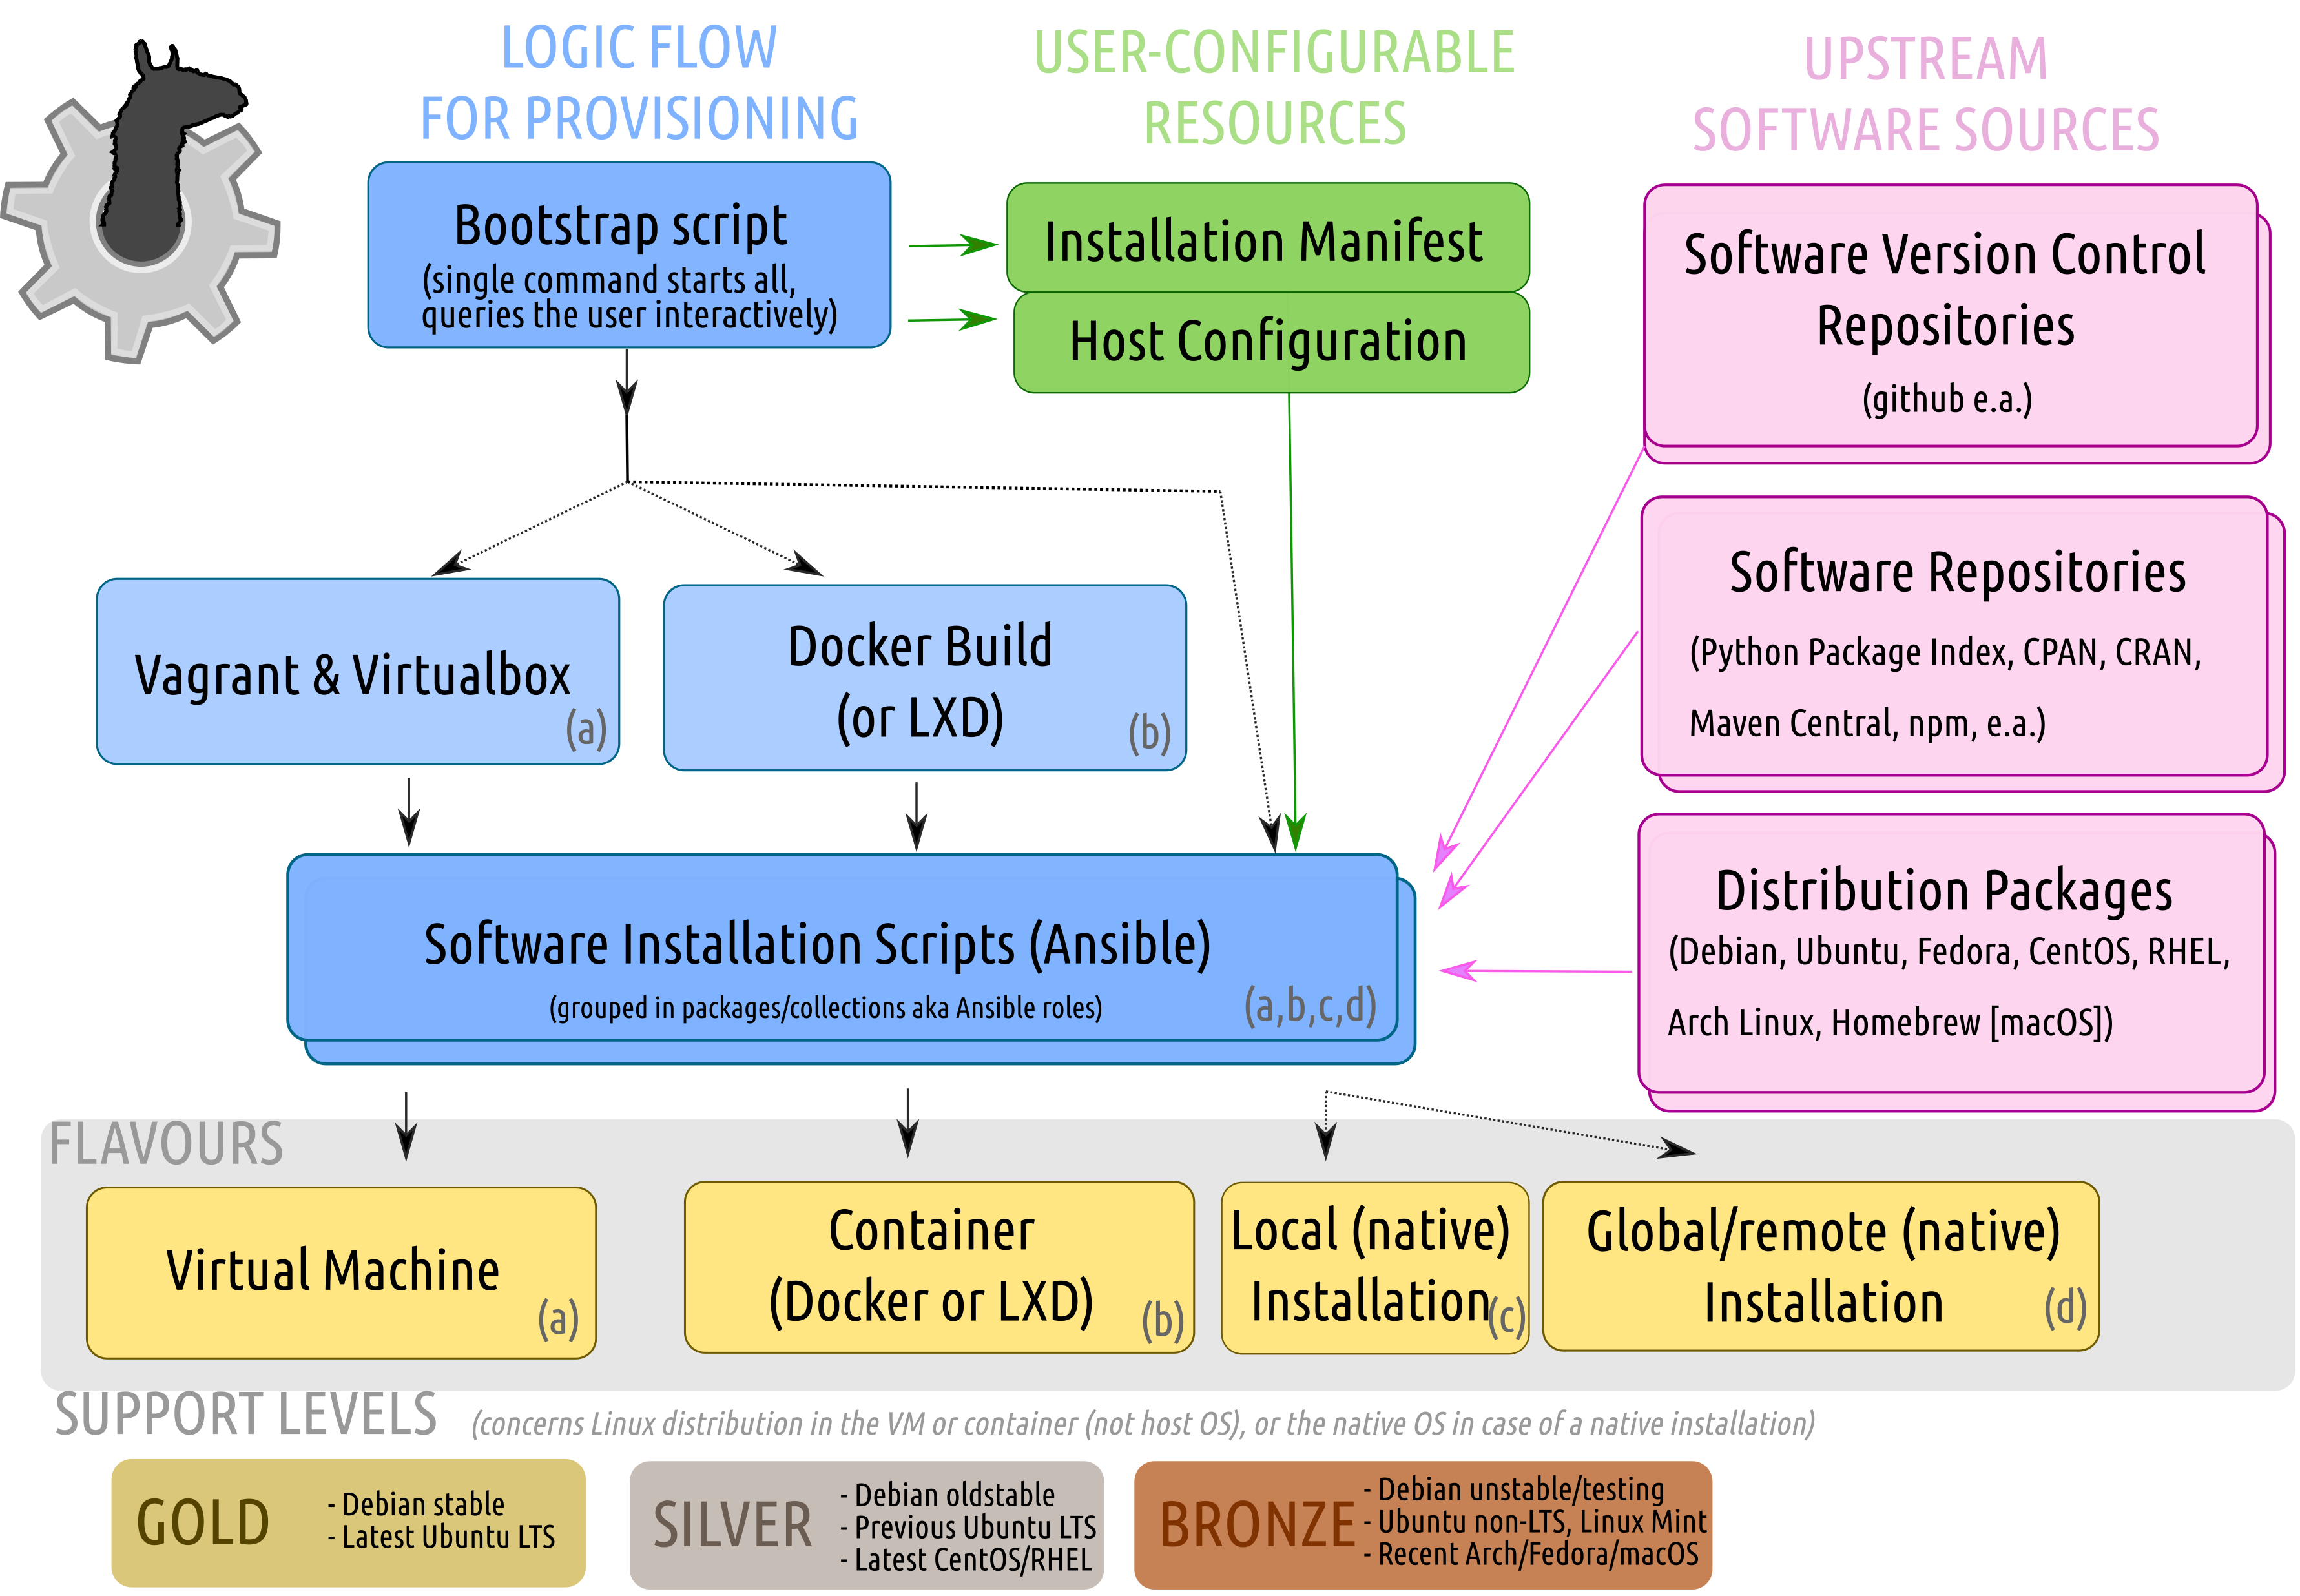
\includegraphics[width=135.0mm]{architecture.png}
\end{center}
\caption{\footnotesize{A schematic representation of the LaMachine architecture}}
\label{fig:arch}
\end{figure}

Once LaMachine is installed, in any of its flavours, it can be updated from inside by running
\texttt{lamachine-update}. This updates all of the software managed by LaMachine.

\subsection{Metadata}
\label{sec:metadata}

LaMachine aims to harmonise the metadata of all installed software. This is accomplished by converting metadata from upstream repositories,
i.e. the repositories where tool providers deposit their software, to a common yet simple standard called CodeMeta
\footnote{\url{https://codemeta.github.io/}, described in JSON-LD} \cite{codemeta,codemetar} where possible, or
encouraging software developers to provide their codemeta metadata inside their source code repositories and using that
directly. CodeMeta is a linked data initiative that provides a mapping from/to various commonly used software metadata
standards\footnote{such as DOAP, Github API, Debian packages, Python distutils, R packages, Ruby gems, Maven metadata, DataCite, WikiData}.
All this metadata in LaMachine in turn enables other tools to do proper service discovery and provenance logging.

The software metadata discussed here is of a generic and practical nature, it most importantly contains information regarding the version, source,
licensing, and authors of the software. The underlying principle is to obtain sofware metadata from as close to the
source as possible. This can be contrasted with other metadata efforts, also within CLARIN, to establish a more
centralised metadata store\footnote{such as CLARIN's CMDI Component Registry;
\url{https://www.clarin.eu/content/component-metadata}} with more specialised and
research-oriented metadata. There is merit to both approaches as they serve distinct functions. But in order to best
serve everybody's different metadata needs, these bottom-up and top-down processes need to come to some kind of
synthesis, e.g. by having component registries do automatic harvesting of CodeMeta (or other) metadata, similar to what LaMachine
does.

\FloatBarrier



\section{Interfaces and Audiences}

We already addressed the need for different interfaces for different audiences in Section~\ref{sec:intro}. The challenge we
face, and for which LaMachine offers a solution, is one of software maintainability, distribution and deployment. How do
we maintain, distribute, and deploy software that is often highly complex and consists of multiple interconnected components, considering
that this software is used differently by different audiences? A key aspect here is the reusability and accessibility of individual
software components. The philosophy we subscribe to encourages the development and distribution of software in a layered or modular fashion,
allowing each building block to serve as the foundation for another more high-level interface, without sacrificing the usability of the
foundation as such. This is in line with the UNIX philosophy of developing tools that do \emph{"one thing only, and do
it well"} and is contrasted with monolithic software solutions that are limiting because they either provide only high-level interfaces but do not
expose their inner components to build upon, or they are as a swiss-army knife full of needless but inseparable
components.

\subsection{Low-level Interfaces}

In any of its flavours, LaMachine offers low-level shell access, i.e. a command-line interface accessed through a
terminal. In flavours that are separated from the host system by a network, this is accomplished over \texttt{ssh}.
After accessing the LaMachine environment through a terminal, as shown in Figure~\ref{fig:venv}, the user has the liberty to do whatever she wants and can invoke any
of the tools that offer a text interface, including text editors such as vim, emacs or nano, version control systems
such as git and interpreters such as Python or R (or compilers for that matter). This allow users to use
one of the many specialised programming libraries included in LaMachine to build their own tools and . All this makes
LaMachine ideally suited as a development environment.

\begin{figure}[htb] \begin{center}
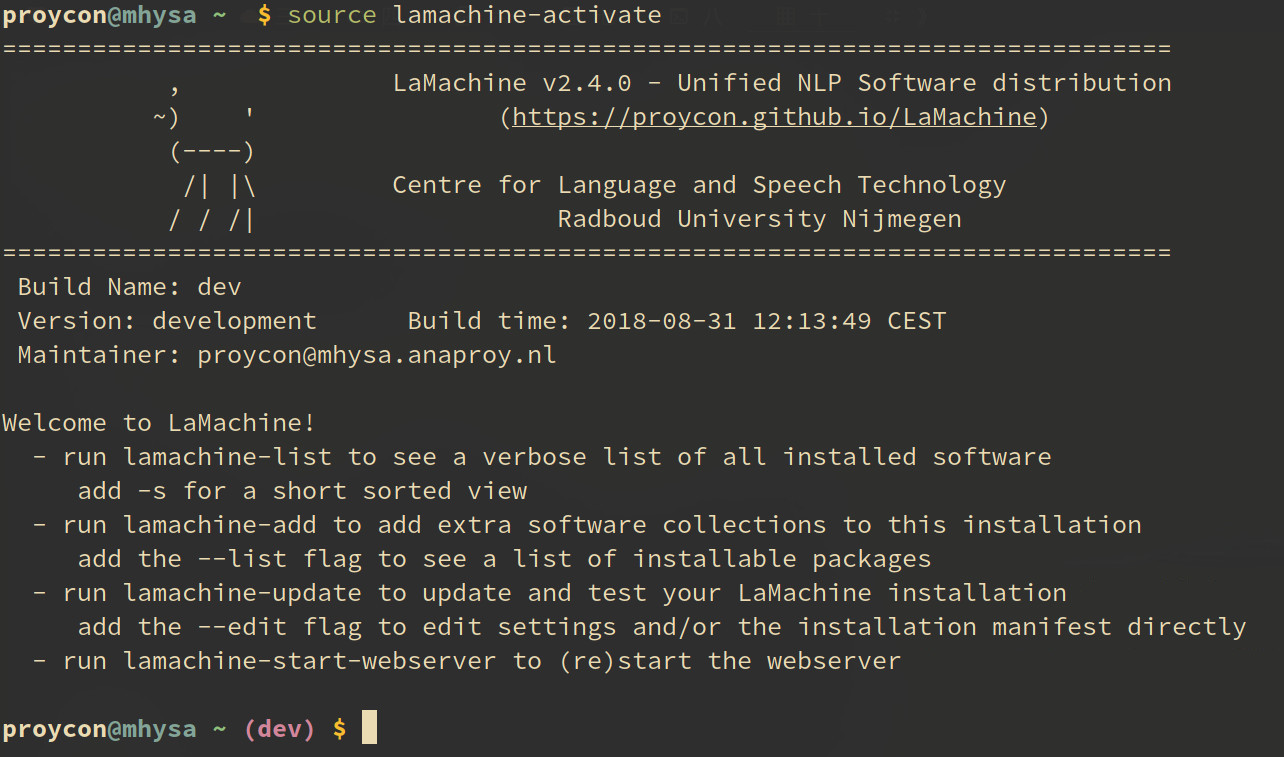
\includegraphics[width=135.0mm]{screenshot_venv_activate.jpg}
\end{center}
\caption{\footnotesize{Activation of a local LaMachine environment on the command-line}}
\label{fig:venv}
\end{figure}

\subsection{High-level Interfaces: Web-based access}

LaMachine comes with a webserver\footnote{In situations where web interfaces are not needed or desired, the
user has the ability to opt-out of this.}. This webserver serves various web-capable tools that are incorporated in LaMachine. One
of these tools is a portal website that provides an overview of all installed software, and acts as a point of access to
all its web services and web applications. This portal, as shown in
Figure~\ref{fig:portal}, leverages the metadata registry compiled in each LaMachine installation (see
section~\ref{sec:metadata}).

\begin{figure}[htb] \begin{center}
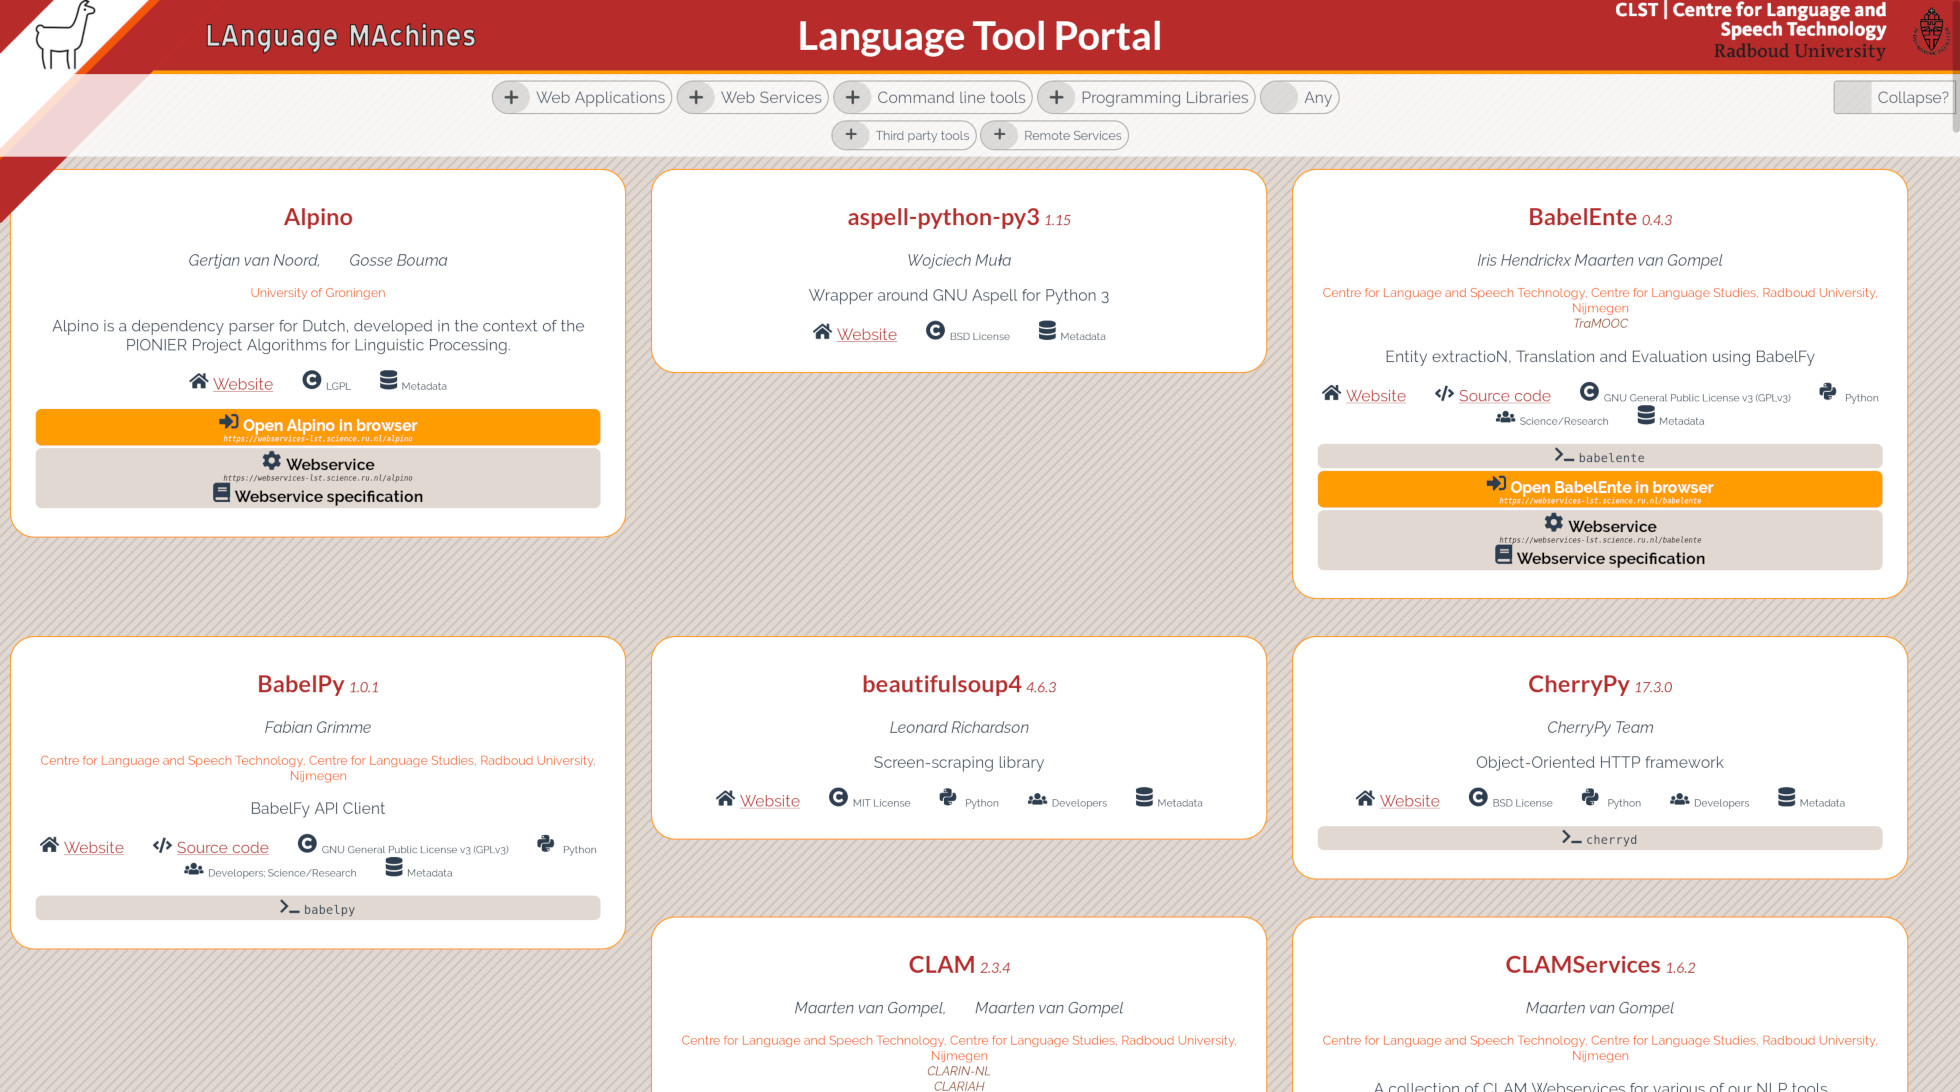
\includegraphics[width=135.0mm]{screenshot_portal.jpg}
\end{center}
\caption{\footnotesize{A screenshot of the LaMachine portal, powered by Labirinto:
\url{https://github.com/proycon/labirinto}}}
\label{fig:portal}
\end{figure}

LaMachine also comes with a
Jupyter Lab\footnote{\url{https://jupyter.org/}} installation which provides a web-based Integrated Development
Environment (IDE) for scripting in Python and R, web-based terminal access, and so-called \emph{notebooks} which mix
text, code and data output and have gained great popularity in the data science community. This is shown in
Figure~\ref{fig:lab}. This type of virtual laboratory provides a powerful interface that provides an alternative to
regular shell access and may have a larger appeal for those parts of the audience that do not feel completely
comfortable in the terminal.

\begin{figure}[htb] \begin{center}
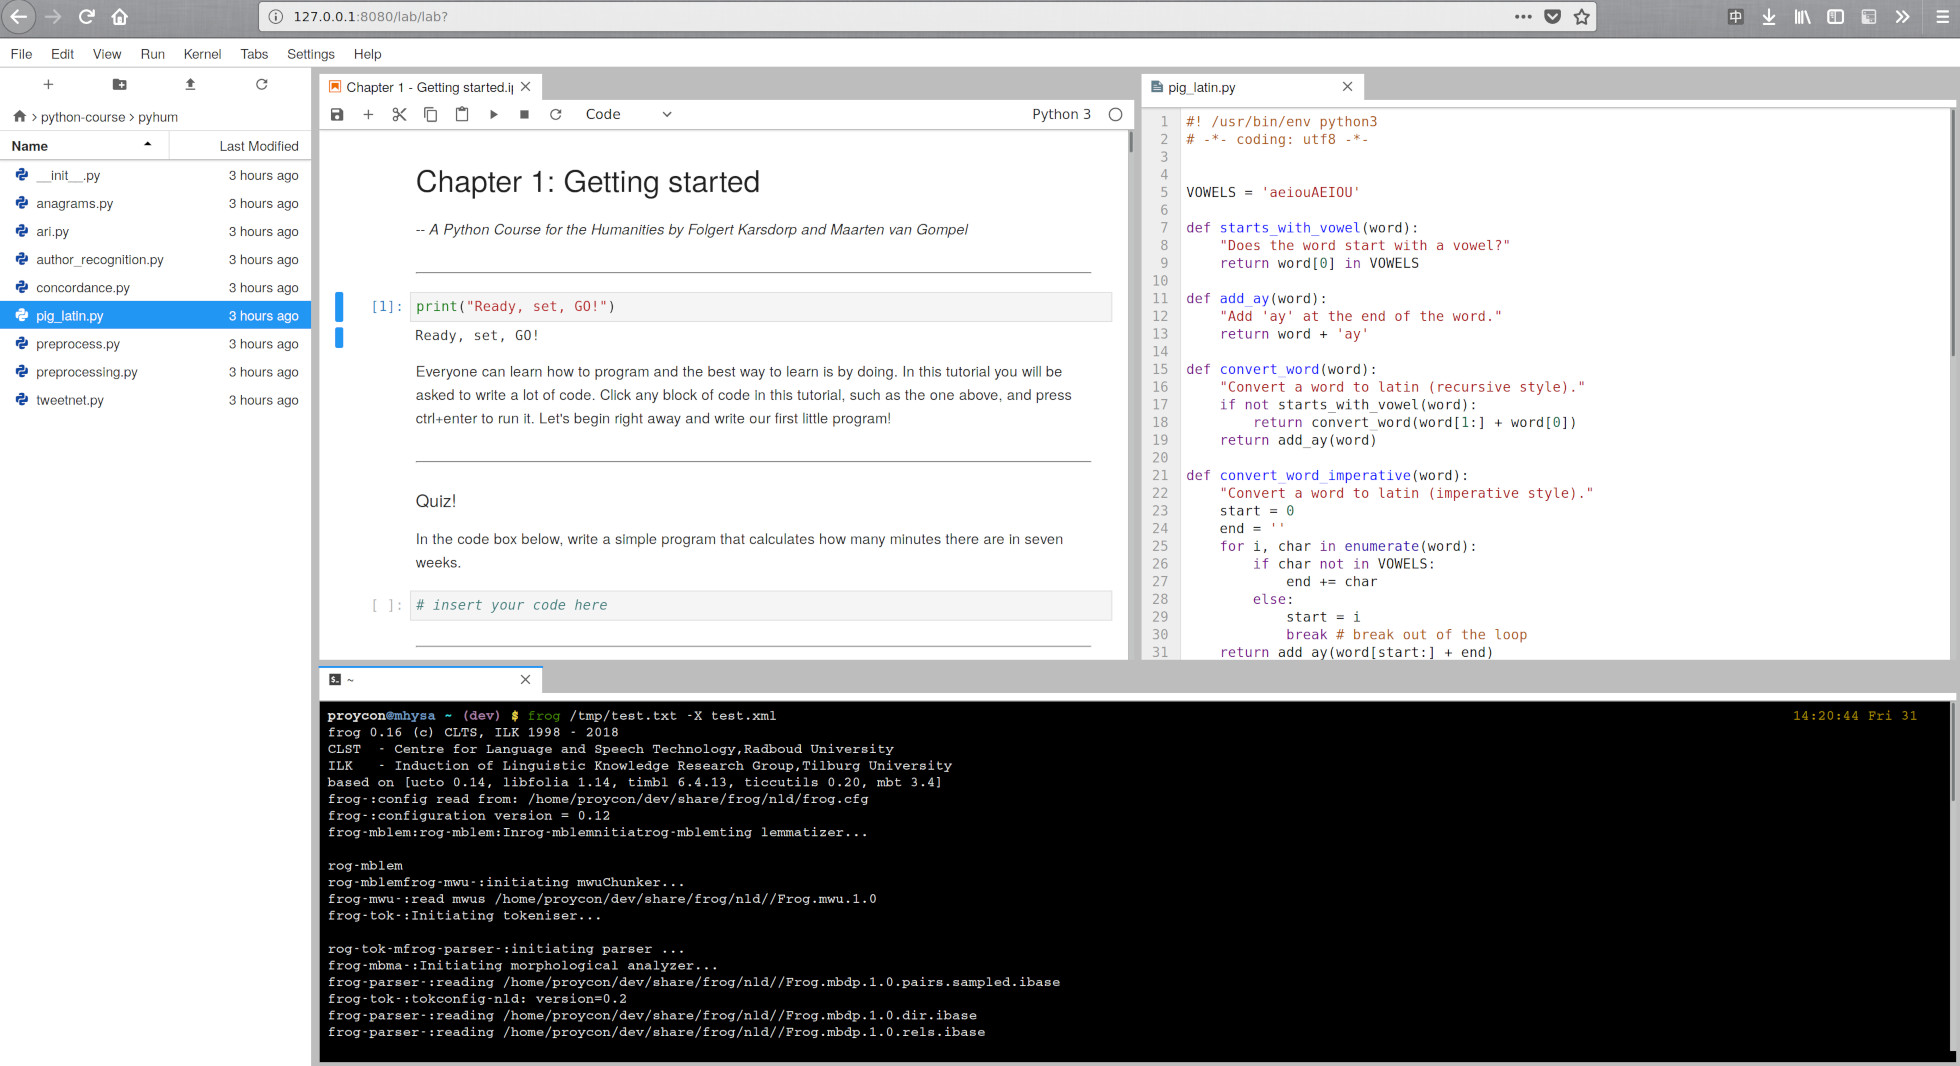
\includegraphics[width=135.0mm]{screenshot_lab.jpg}
\end{center}
\caption{\footnotesize{A screenshot of the Jupyter Lab Environment}}
\label{fig:lab}
\end{figure}

LaMachine provides various CLAM-based webservices. CLAM is a long-time CLARIN project that allows developers to turn
their command-line NLP tool into a RESTful webservice with relatively little effort \cite{CLAMPAPER}, and which in
addition also provides a generic web-interface for human end-users. The portal website in LaMachine links to these. This
again addresses an audience that does not require a high degree of technical expertise, but is suitable for a wider
audience of researchers, including those in the Humanities.

\section{Comparison to alternative distributions}
\label{sec:comparisons}

How does LaMachine compare to alternatives? To answer this question we must first look at what may be considered
alternatives to LaMachine. At this point, it is important to emphasise once more that LaMachine is offered as convenience.
LaMachine always seeks to use installation channels that the user can also access directly. For instance, is the user
only interested in a single Python package that LaMachine offers? Then she can just as well install it directly using
\texttt{pip install}. Is the user only interested in a single package that  the underlying Linux distribution (or
macOS's homebrew)
already provides? Then, by all means, she should go for that.

LaMachine starts to fill a need when the user is interested in complex software, such as complex NLP pipelines with
multiple components, the individual installation (sometimes involving compilation from source) and configuration of
which would be not be trivial. Moreover, LaMachine shines when the user wants higher-level interfaces on top of that,
something she can use right out of the box. It also fulfills a role in case the user simply does not know what she wants
or needs yet, and needs an environment where she can explore a variety of pre-installed tools and experiment.

Comparisons could be drawn between LaMachine as a kind of Linux distribution and other Linux distributions. But that
would not be appropriate as we characterise LaMachine more as a meta-distribution which simply builds on the foundation
of several existing major Linux distributions. As a meta-distribution that runs in a variety of flavours and on a
variety of platforms, it offers a great deal of flexibility that normal distributions do not have. At the same time, the scope of
LaMachine is more narrowly defined than that of a generic Linux distribution, including even specialised Linux
distributions that focus on scientific computing, such as Fedora
Scientific\footnote{\url{https://labs.fedoraproject.org/en/scientific/}}.

The best comparison can perhaps be drawn with Anaconda\footnote{\url{https://www.anaconda.com/}}, which we could also qualify as
a meta-distribution under our definition, and which enjoys great popularity in the data science community. Anaconda has
a focus on Python and R. It is much wider in scope than LaMachine, which has a strong NLP and CLARIN/CLARIAH focus. When
it comes to Python, which Anaconda is initially geared at, there is considerable overlap in the modules that LaMachine and Anaconda offer. Unlike LaMachine,
Anaconda does not focus on providing different flavours such as a VM or a Docker Container\footnote{This is not a
technical limitation but simply a matter of different objectives, one could easily create a VM or Docker Container and
install Anaconda in it.}, nor separate stable and development versions of the included software.

At the start of the development cycle for LaMachine v2, we investigated whether Anaconda and its ecosystem would provide
a sufficient foundation for us to build upon. We concluded this was not the case for a number of reasons: Anaconda
introduces more overhead than we desired for our purposes and conflicted with certain technology choices we made. We
wanted our native flavours (local environment and global environment) to be as close to the underlying distribution as possible and to reuse existing
technologies and packages, such as compilers (e.g. gcc) and
interpreters (e.g. python), from the distribution (or from homebrew for macOS).  Anaconda, on the other hand, choses to provide its own packages and builds on those. It
does so using its own package manager (conda) and package repositories (conda-forge). This would require repackaging certain software for the
anaconda ecosystem.

For the distribution and deployment of complex software setups such as NLP pipelines, containers are a common solution
nowadays. The Docker flavour of LaMachine provides something similar, but rather than providing a single static Docker recipe
that builds a single kind of container, LaMachine offers a high degree of flexibility for the construction of different
containers, i.e. containing different software of having different configurations, based on the user's needs. It is
quite feasible to instantiate a variety of LaMachine containers and use a container orchestration system such
Kubernetes or Docker Swarm for automated deployment, scaling and management thereof. Such orchestration, however, is
beyond the scope of LaMachine itself, which aims to provide a singular environment, i.e. everything installed in a
LaMachine instance shares the same userspace and duplication is strongly minimised.

The flexibility LaMachine offers, with various flavours and versions, makes it more accessible and deployable in
multiple contexts, but this does come at a cost. Maintaining LaMachine itself is a non-trivial task that requires
constant maintenance and testing\footnote{We run automated tested on a continuous integration platform to this end};
software exists in an ever moving ecosystem. Any of the distributions we target, or software that participates, \emph{might}
at any time introduce a change that requires us to adapt LaMachine accordingly. Similarly, underlying Linux
distribution releases that are currently up-to-date and supported, will eventually be deprecated and replaced by newer releases, a development
LaMachine is obliged to follow by design.

\section{Case studies}\label{sec:case}

\subsection{Text Mining for Health Inspection}


We participated in a small Dutch national project titled \emph{``Text mining for Inspection: an exploratory study on
automatic analysis of health care complaints''} \footnote{\url{https://bit.ly/2N2AICS}} %links to https://www.zonmw.nl/nl/onderzoek-resultaten/kwaliteit-van-zorg/program/project-detail/effectief-toezicht/tekstmining-in-het-toezicht-een-exploratieve-studie-naar-de-automatische-verwerking-van-klachten-in/}.
led by IQhealthcare\footnote{\url{http://www.iqhealthcare.nl/nl/}}, the scientific centre for healthcare quality of RadboudUMC hospital.
This project took place at the Dutch Health Inspectorate and aimed to apply text mining techniques to health care
complaints that have been registered at the national contact point for health care (Landelijk Meldpunt
Zorg\footnote{\url{https://www.landelijkmeldpuntzorg.nl}})
We investigated the usefulness of text mining to categorise and cluster complaints, to automatically determine the
severity of incoming complaints, to extract patterns  and to identify risk cases. This project turned out to be a good
test case of the applicability and usefulness of LaMachine as a standalone research environment.
As the complaint data is highly sensitive, it could not leave the secure servers of the health inspectorate and was
stored in an environment without internet access. We needed to bring the software to the data via a shared folder.

We used a virtual machine (VM) image of LaMachine and we ran this 64-bits Linux-based VM inside another
VM with Windows Server 2012, provided to us by the health inspectorate for this project, in which we did have administrative
rights but no internet access. In terms of hardware we ran on a machine with 8 cores and  32GB internal memory available.
%using VirtualBox and Vagrnt on the Windows VM
LaMachine provided a fully functional research environment and we ran all our experiments within LaMachine. We interacted with LaMachine both through the command line, which offers a standard
shell and enables access to all lower-level tools and programming languages; and through the (offline) webbrowser to use
the Jupyter Notebook environment.

LaMachine comes with some simple data sharing facilities that allowed us to access the sensitive complaint data via a
single shared dataspace between host and the VM. Extensive data search and management functions are deliberately beyond the scope of LaMachine, and left to more high-level tooling.

We used many of the available tools in LaMachine within this project: Frog for linguistic annotation of the textual
content of the complaint and the scikit-learn Python package for classification, T-scan for feature extraction in the form of text characteristics and colibri-core for n-gram analysis.

%het doel van deze studie is om automatische tekstanalysetechnieken (tekstmining) toe te passen op de klachten die bij het Landelijk Meldpunt Zorg binnenkomen. Zo hopen we eventuele trends en patronen te vinden die meer inzicht geven in de aard en de relevantie van de klachten. De verwachting is om zo potentiële risicogevallen te ontdekken die op basis van de behandeling van individuele klachten nog niet waren gesignaleerd.

\subsection{Workshop: Cataloguing of Textual Cultural Heritage Objects}
\label{sec:case2}

The ICT-Research Platform Netherlands and NWO organise a yearly one-week workshop `ICT with Industry'
\footnote{https://ict-research.nl/ict-with-industry/ictwi2019/} to stimulate collaboration between industry and
academia. The industrial partner provides a problem and a team of researchers from different backgrounds and
universities collaborate to come up with solutions. We participated in the 2019 edition on the case study by the Dutch Royal Library who wanted to investigate automatic methods for cataloguing of textual cultural heritage objects, in this particular case a large collection of digital dissertations.

For this workshop, computing power was purchased at SURFsara, a collaborative organization for ICT in Dutch education
and research. Subsequently, we had the ability to create Virtual Machines on their hosting platform. For this workshop
we had twelve participants and decided to create a single multi-core and high memory VM to share amongst the
participants to create one common digital workspace.

As recommended by SURFsara, we opted for one of their default Linux images as a basis for the VM, based on Ubuntu 18.04,
instead of providing a LaMachine VM image directly like we did in~\ref{sec:case}. This was recommended because their image
was already preconfigured to integrate nicely with their cloud environment. Inside this VM we simply bootstrapped the local
installation flavour of LaMachine.  Here we benefit from the flexibility LaMachine offers because of its various
flavours, and regardless of the flavour, the resulting installations are always functionally equivalent. The local
environment flavour had the added bonus of not being in anyone's way in case any of the twelve workshop participants did
not want to use LaMachine, considering it needs to be explicitly activated prior to usage.

LaMachine offered a convenient platform for a range of different explorations and experiments in the area of NLP and
text mining.  However, for some situations LaMachine, or rather Linux in general, was not a good fit for the audience of
the workshop: For team members who did not have experience with a non-Windows environment, LaMachine was not a suitable
or useful tool. The limit of LaMachine was also reached for members who wanted to use desktop text editors with a
graphical user interface as this is not offered by LaMachine. Moreover, we did not manage to get X-forwarding working in the
Ubuntu Linux VM and after a few attempts the team gave up on resolving this issue due to time pressure. This, also
demonstrates that fine-tuning the configuration of certain aspects of LaMachine, but especially beyond LaMachine, is beyond the reach of a data scientist
without system administration skills. This certainly also applies also to the installation as a whole in the
SURFsara context, which involved things like the partitioning, formatting and mounting of (virtual) drives and setting
up user accounts on the shared VM, all of which require some system administration skills and are too context-specific
to be within the scope of LaMachine.
Lamachine was convenient and speeded up writing code as the most common scientific data-related packages are already present in Lamachine.
 %verwerkt <-- <iris> it moet nog wat beter geformuleerd worden maar je snaprt wat ik bedoel
%@iris: hebben jullie verder geen gebruik proberen te maken van de Jupyter Lab omgeving? Dat biedt in ieder geval iets
%grafisch wat via web te benaderen is?
%@maarten helaas lukte dat ook niet, dat liep bij mij steeds vast. - ik heb opmerking van alex over tijdswinst toegevoefd

\section{Conclusion \& Future work}

LaMachine provides a flexible solution for the installation of a variety of NLP software, resulting in a kind
of virtual laboratory that, through various interfaces, can be employed by a variety of people, from developers and data scientists to the wider research community that CLARIN explicitly addresses.

Use cases as the examples in section \ref{sec:case} contribute to thorough testing and running of LaMachine in less ideal
circumstances such as nested VM constructions and offline usage.

Aside from the incorporation of new relevant software, the main objectives for the future are to provide
greater \emph{interoperability} between the included tools through better \emph{high-level interfaces} for the
researcher. We see this as a bottom-up process and have now established a firm foundation to build upon. Note that such
proposed interfaces, including the current portal application in LaMachine, are always considered separate independent
software projects, which may be deployed by/in/for LaMachine, but also in other contexts. LaMachine remains `just'
a software distribution at heart.

Development of LaMachine presently takes place in collaboration with the CLARIAH WP3 Virtual Research Environment (VRE)
project\footnote{\url{https://github.com/meertensinstituut/clariah-wp3-vre}}, which has higher ambitions in
accommodating the researcher and connectivity of data and services, and transcends also those of the CLARIN Language
Resource Switchboard~\cite{switchboard}. An important part of our future focus will therefore be on interoperability
with the higher-level tools emerging from the VRE efforts, but also with other parts of the CLARIN infrastructure;
single-sign on authentication being a notable example here.

LaMachine v2 is open to  outside contribution. Contributor documentation has been written, and at this stage, we greatly
welcome external participants to join in.

\section*{Acknowledgement}

This research was funded by NWO CLARIN-NL, CLARIAH and the ZonMw project {\it Tekstmining in het toezicht: een exploratieve studie naar de automatische verwerking van klachten ingediend bij het Landelijk Meldpunt Zorg}, project number 516004614. We thank the Dutch Health Inspectorate, IQhealthcare, and Tim Voets for their valuable contributions and help in the ZonMw project, and NWO, the ICT Research Platform Nederland, the Lorentz Centre, the Royal Library and all our team members for making the ICT with Industry workshop a success.


\bibliography{lamachine}



\end{document}

